\documentclass[ebook,article,11pt]{memoir}

% \usepackage{setspace}

\usepackage{mdframed}
\usepackage{graphicx}
\usepackage{hyperref}

\definecolor{myblue}{RGB}{190,190,255}

\newmdenv[backgroundcolor=myblue,roundcorner=2pt,skipabove=3pt,skipbelow=3pt,%
          hidealllines=true,font=\small,splittopskip=0.45cm,splitbottomskip=0.1cm]{block}

% \usepackage{tikz}

% \tikzstyle{block} = [rectangle, thick, fill=myblue, text width=\textwidth - 0.2cm, %<---------= 
%              rounded corners, minimum height=1em, font=\small,
%              minimum width=\textwidth]

% \usetikzlibrary{shadows}


\pagestyle{myheadings}

\renewcommand{\rmdefault}{ppl}
% \setstretch{1.5}

\author{Daoud Clarke, ChatbotTech.io\\
  \\
  Copyright Hyperparameter Limited 2018}

\title{\textbf{Let's Chat about Chatbot Tools}}

\date{}

\begin{document}

\maketitle

\chapter{Introduction}
\markboth{Introduction}{Introduction}

It seems like every day there is a new chatbot tool. While building a
chatbot is becoming easier and easier, knowing which is the
\emph{best} tool for you is becoming harder and harder, simply because
there are so many tools.

ChatbotTech.io was created to solve this problem. We've reviewed the
most popular tools, so you don't have to. Each tool is reviewed and
rated, so you can quickly find the best tools and see which ones are
likely to work for you. I have personally tried out each tool reviewed
here, and I can tell you, they are not all the same! Some are good and
some are sad and some are very very bad, to paraphrase Dr Seuss. When
they're bad, I won't be afraid to say so.

\section*{Too long, didn't read}

Because there are so many tools, it's hard to know where to
start. Well, start here!

\begin{center}
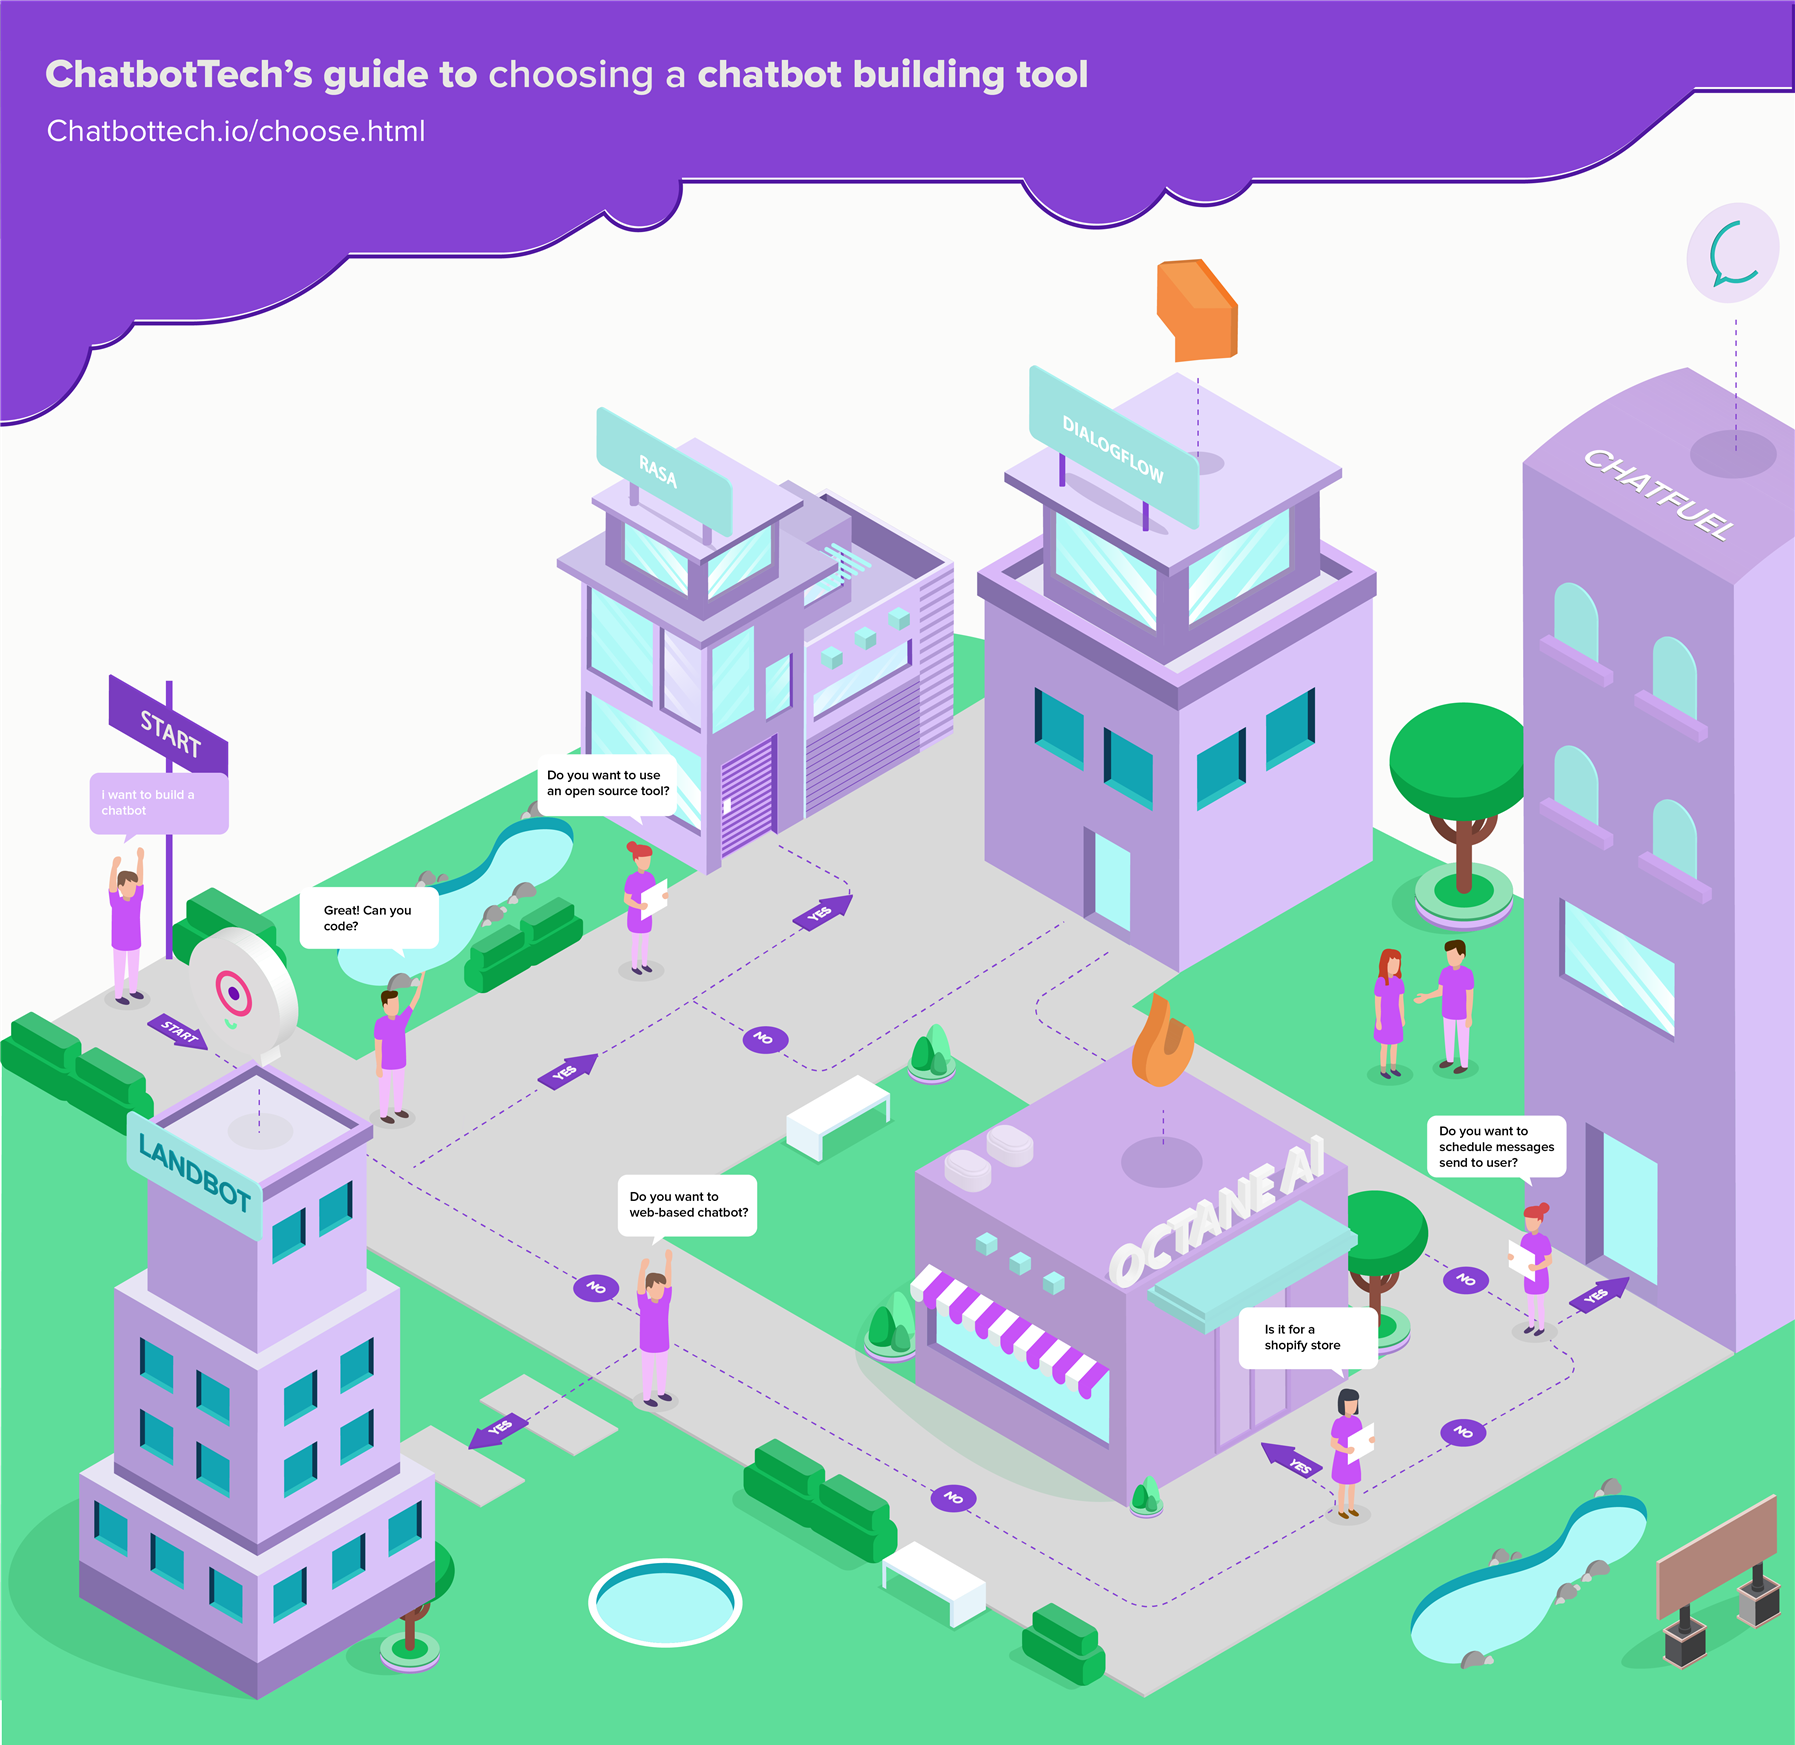
\includegraphics[width=\textwidth]{guide.png}
\end{center}

The chances are, one of these top tools will be right for you:
\begin{itemize}
\item \textbf{Chatfuel} is great for quickly getting a Messenger
  chatbot together if you don't have any technical skills and don't
  need to handle complex queries.
\item \textbf{Dialogflow} has sophisticated natural language
  processing abilities for answering user queries
\item \textbf{Rasa} is open source which may be useful if you want to
  host the bot yourself. It can also handle more complex queries, like
  Dialogflow, but the quality is not quite as good.
\item \textbf{Landbot} is another non-technical tool which is great
  for creating a web-based chatbot.
\item \textbf{Octane AI} is aimed at users with a Shopify site that
  want to provide their users with a chatbot.
\end{itemize}

Check out the reviews later in the book for details. If none of these
seem right, read on! There are plenty more to choose from.

\chapter{Chatbot Tool Reviews}

\input{collated.tex}

\vspace{0.5cm}
\noindent
\begin{block}
\texttt{daoud@hyperparameter.com}
\end{block}
\end{document}
